\documentclass[11pt, a4paper]{article}

\usepackage[T1]{fontenc}
\usepackage[utf8]{inputenc}
\usepackage[english]{babel}
\usepackage{lmodern}
\usepackage{microtype}
\usepackage[top=2.0cm, bottom=2.2cm, left=1.8cm, right=1.8cm]{geometry}
\usepackage{booktabs}
\usepackage{float}
\usepackage[table]{xcolor}
\usepackage{hyperref}
\hypersetup{colorlinks=true, linkcolor=darkblue, citecolor=darkblue, urlcolor=darkblue}
\usepackage{graphicx}
\usepackage{titlesec}
\usepackage{fancyhdr}
\usepackage{parskip}
\usepackage{amsmath}
\usepackage{amssymb}
\usepackage{tikz}
\usetikzlibrary{arrows.meta, positioning}
\usepackage{caption}
\captionsetup{font=small, labelfont=bf}

\definecolor{darkblue}{RGB}{26, 60, 120}

\titleformat{\section}
  {\large\bfseries\color{darkblue}}
  {\thesection.}{0.6em}{}[\vspace{-4pt}\rule{\linewidth}{0.4pt}]

\titleformat{\subsection}
  {\normalsize\bfseries\color{darkblue}}
  {\thesubsection}{0.6em}{}

\pagestyle{fancy}
\fancyhf{}
\fancyhead[L]{\small\textcolor{gray}{TER -- Monthly Report}}
\fancyhead[R]{\small\textcolor{gray}{M1 MLDM -- UJM Saint-Etienne}}
\fancyfoot[C]{\small\thepage}
\renewcommand{\headrulewidth}{0.3pt}

\setcounter{secnumdepth}{2}

\begin{document}

\begin{titlepage}
    \centering
    \vspace*{1.5cm}
    {\large\color{darkblue}\textbf{Universite Jean Monnet Saint-Etienne}}\\[0.3em]
    {\normalsize TER -- S2 2025/2026}

    \vspace{1.5cm}
    {\color{darkblue}\rule{\linewidth}{1.5pt}}
    \vspace{0.6cm}

    {\LARGE\bfseries\color{darkblue} Design and Evaluation of a Legal AI Assistant:\\
    A Comparative Study of RAG and Fine-Tuning}

    \vspace{0.4cm}
    {\large Monthly Progress Report -- June/July 2026}
    \vspace{0.6cm}

    {\color{darkblue}\rule{\linewidth}{1.5pt}}
    \vspace{1cm}

    
\includegraphics[width=0.4\linewidth]{latex_assets/UJM-LOGO-NOIR.png}
    \vspace{1.5cm}

    {\large\bfseries Author}\\[0.8em]
    \begin{tabular}{c}
        {\large Chaabane Ouammou} \\[0.3em]
        \small M1 MLDM\\
    \end{tabular}

    \vspace{0.6cm}
    \begin{tabular}{c}
        {\normalsize Co-author: Bartosz Konior} \\[0.2em]
        \small M1 DSC\\
    \end{tabular}

    \vspace{1cm}
    \begin{tabular}{rl}
        \textbf{Advisor:} & Marc Sebban \\[0.3em]
    \end{tabular}
\end{titlepage}

\pagecolor{white}
\color{black}
\setcounter{page}{1}
\twocolumn

\section{What This Month Was About}

The previous report left the project with a first working version of both pipelines and a single comparison between them, run on a small sample of questions. This month was spent going back over almost every part of that first version one piece at a time, checking what still held up under closer scrutiny and what did not, and building the pieces that were still missing, most importantly a proper statistical comparison and a human evaluation. The order below roughly follows the order the work actually happened in, starting with retrieval since everything else in the RAG pipeline depends on it.

\section{Going Back Over Retrieval}

Retrieval decides which statutory articles the generator gets to see, so before touching anything else it seemed worth checking how good it really was. The general purpose sentence embedding model used previously was replaced with a larger multilingual model, \texttt{multilingual-e5-large}, and a lexical BM25 baseline was added alongside it, together with a simple hybrid that combines the two rankings. The idea was to see how much of the earlier weak retrieval was really a limit of the dataset and how much was just the embedding model not being strong enough.

\begin{figure}[H]
\centering
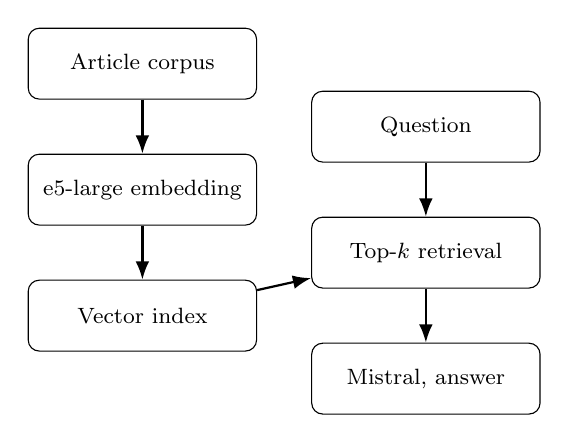
\begin{tikzpicture}[
  box/.style={draw, rounded corners, minimum height=0.9cm, minimum width=2.9cm, align=center, font=\footnotesize, inner sep=4pt},
  arr/.style={-{Latex}, thick}
]
\node[box] (corpus) at (0,2.4) {Article corpus};
\node[box] (embed)  at (0,0.8) {e5-large embedding};
\node[box] (index)  at (0,-0.8) {Vector index};
\node[box] (question) at (3.6,1.6) {Question};
\node[box] (retrieve) at (3.6,0) {Top-$k$ retrieval};
\node[box] (answer)   at (3.6,-1.6) {Mistral, answer};
\draw[arr] (corpus) -- (embed);
\draw[arr] (embed) -- (index);
\draw[arr] (index) -- (retrieve);
\draw[arr] (question) -- (retrieve);
\draw[arr] (retrieve) -- (answer);
\end{tikzpicture}
\caption{Retrieval pipeline. The corpus is indexed once, a question is compared against it at inference time, and the retrieved articles are added to the prompt.}
\label{fig:ragdiagram}
\end{figure}

\begin{table}[H]
\centering
\small
\begin{tabular}{lccc}
\toprule
\textbf{Method} & \textbf{R@1} & \textbf{R@5} & \textbf{R@10} \\
\midrule
BM25 & 0.063 & 0.184 & 0.224 \\
mpnet (previous) & 0.021 & 0.074 & 0.097 \\
e5-large & 0.083 & 0.211 & 0.296 \\
Hybrid BM25+e5 & 0.106 & 0.250 & 0.322 \\
\bottomrule
\end{tabular}
\caption{Retrieval quality on the full 222 question test set.}
\label{tab:retrieval}
\end{table}

The upgrade helps clearly, Recall@1 roughly triples and the hybrid combination pushes every score up a little further still, so the earlier weak retrieval was at least partly a matter of which embedding model had been chosen rather than a hard limit of the dataset. Even so, the correct article is still missed more than two thirds of the time within the top ten results, which is not a small gap and is picked up again later in this report.

One thing is worth flagging honestly rather than passed over. The Recall@10 obtained here for e5-large, 0.296, is noticeably lower than what an earlier evaluation of the same kind of model had suggested. Checking whether long articles being cut off could explain this did not turn up a convincing answer, most articles are short. Two other explanations remain possible and have not been tested yet, that the earlier index may have included extra text such as the code and chapter headings, or that it may have relied on a retriever adjusted slightly on the dataset rather than used exactly as published. This is left open rather than picking one explanation without checking it first.

\section{Extending the Fine-Tuning Runs}

The previous fine-tuning result came from a single run, which left open how much of it depended on the particular random seed, or on choices such as the adapter rank or how much training data was used. This month, with a somewhat larger training set available, that single run was turned into a small family of runs changing one thing at a time.

Fine-tuning still works by freezing the base model and adding a small trainable adjustment to a few of its weight matrices rather than retraining the whole network, which is what makes it possible to run on a single consumer GPU. The adapter rank, which controls how large that adjustment is allowed to be, was raised from 16 to 32 this month, trained on 580 questions instead of 380.

\begin{figure}[H]
\centering
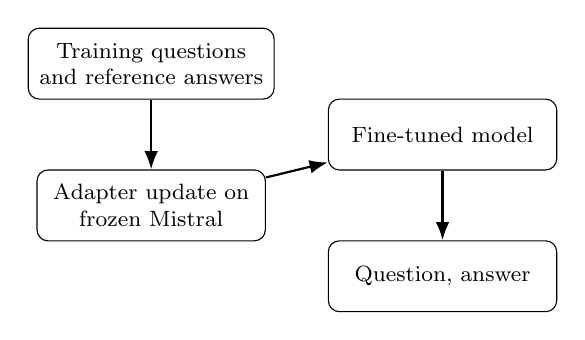
\begin{tikzpicture}[
  box/.style={draw, rounded corners, minimum height=0.9cm, minimum width=2.9cm, align=center, font=\footnotesize, inner sep=4pt},
  arr/.style={-{Latex}, thick}
]
\node[box] (pairs)  at (0,1.4)  {Training questions\\and reference answers};
\node[box] (lora)   at (0,-0.4) {Adapter update on\\frozen Mistral};
\node[box] (tuned)  at (3.7,0.5) {Fine-tuned model};
\node[box] (answer) at (3.7,-1.3) {Question, answer};
\draw[arr] (pairs) -- (lora);
\draw[arr] (lora) -- (tuned);
\draw[arr] (tuned) -- (answer);
\end{tikzpicture}
\caption{Fine-tuning pipeline. Only the small adapter is trained, the base weights never change, and no retrieval step is involved at inference time.}
\label{fig:ftdiagram}
\end{figure}

A change made specifically this month was adding a small validation set, 100 questions kept aside with a fixed seed, since the previous run had no way of telling whether the model was really learning to generalize or simply memorizing 380 examples. With that validation set in place it became possible to compare rank 16 against rank 32, attention only against attention plus feed forward layers, and different amounts of training data, on a signal that actually reflects generalization rather than training loss alone.

\begin{table}[H]
\centering
\small
\begin{tabular}{lccc}
\toprule
\textbf{Variant} & \textbf{$n$} & \textbf{Train loss} & \textbf{Val loss} \\
\midrule
main (rank 32) & 580 & 0.834 & 0.679 \\
rank 8 & 580 & 0.850 & 0.710 \\
$n=380$ & 380 & 0.966 & 0.860 \\
$n=786$ & 786 & 0.736 & 0.561 \\
attn + MLP & 580 & 0.527 & 0.416 \\
\bottomrule
\end{tabular}
\caption{Selected fine-tuning variants, three epochs each.}
\label{tab:finetune}
\end{table}

More training data helps in a fairly regular way, and letting the adapter touch the feed forward layers in addition to attention lowers the validation loss a lot, though the gap between training and validation loss also grows at the same time, which usually means the model is fitting its training data more closely without a guarantee that this transfers well to new questions. The main configuration was also repeated on three different random seeds, giving a training loss of $0.843 \pm 0.006$, stable enough on its own, though as the next section shows the quality of the actual generated answers varies more across those same three seeds than the training loss alone would suggest.

\section{Comparing Four Configurations Properly}

The earlier comparison used three configurations on 50 questions and a single run. This month a fourth configuration was added, the fine-tuned model combined with retrieval, specifically because there was no way to tell from the earlier setup whether the two techniques help with the same weakness or with different ones, and the comparison was moved to the full 222 question test set with a proper statistical treatment rather than a single number per configuration.

Confidence intervals were obtained by resampling the 222 questions with replacement many times and looking at how much the average score moves around across those resamples, which gives a sense of how much a given score could plausibly have come out different by chance alone. Every pair of configurations was also tested twice for a genuine difference, once with a test on the resampled differences and once with a rank based test that makes fewer assumptions about the data, and a correction was applied to account for testing six pairs at once rather than treating each comparison as if it were the only one being made.

\begin{table}[H]
\centering
\small
\begin{tabular}{lcc}
\toprule
\textbf{Config} & \textbf{ROUGE-L} & \textbf{95\% interval} \\
\midrule
Zero-shot & 0.110 & 0.104 to 0.116 \\
RAG & 0.140 & 0.129 to 0.151 \\
Fine-tune & 0.147 & 0.136 to 0.160 \\
Fine-tune + RAG & 0.179 & 0.157 to 0.202 \\
\bottomrule
\end{tabular}
\caption{ROUGE-L with bootstrap confidence intervals, full test set.}
\label{tab:generation}
\end{table}

\begin{figure}[H]
\centering

\includegraphics[width=\linewidth]{latex_assets/figs/config_comparison_ci.pdf}
\caption{ROUGE-L with confidence intervals for the four configurations.}
\label{fig:configci}
\end{figure}

Adding retrieval or fine-tuning on their own both clearly beat the zero shot baseline. Retrieval and fine-tuning taken separately are not statistically distinguishable from each other, both tests agree on that, which already says the two techniques are closer to each other in overall quality than their raw scores in the table might suggest on their own. The comparison between fine-tuning alone and the combined configuration is the one case where the two tests disagree, so that particular comparison is treated here as unresolved rather than picking the answer that looks better.

The earlier report's fine-tuning result, measured on 50 questions, was noticeably higher than the 0.147 measured here on the full 222 questions, close to the upper edge of the confidence interval in Table~\ref{tab:generation} without quite falling inside it. This is not treated as a mistake to fix, it is a fairly direct illustration of how much a 50 question estimate can move once measured on a larger and more representative set of questions, which is the main reason this whole comparison was redone this month rather than reused as is.

\section{Where the Remaining Error Comes From}

Once retrieval and generation were both stronger, the natural next question was which one was still holding the RAG pipeline back. An experiment was set up to answer this directly, the true relevant articles were placed straight into the prompt without going through the retriever at all, which removes retrieval error completely and shows what the generator alone could achieve if retrieval were perfect.

\begin{table}[H]
\centering
\small
\begin{tabular}{lccc}
\toprule
\textbf{Condition} & \textbf{ROUGE-L} & \textbf{Exact match} & \textbf{Halluc.} \\
\midrule
Zero-shot & 0.110 & 0.005 & 0.144 \\
RAG (real) & 0.140 & 0.036 & 0.234 \\
Oracle context & 0.252 & 0.311 & 0.117 \\
\bottomrule
\end{tabular}
\caption{Oracle context experiment, base model throughout.}
\label{tab:oracle}
\end{table}

The gap between real retrieval and this oracle condition is large on citation accuracy, far larger than the gap between real retrieval and no context at all, which means most of what is currently missing comes from retrieval failing to find the right article rather than from the model failing to use a correct one once it has it. One result was not expected going in, the model hallucinates more with real retrieval than with no context whatsoever, as if a wrong but plausible looking article invites more confident invention than having nothing to work from. The same protocol was also run once on Qwen2.5-7B-Instruct instead of Mistral, mainly to check this was not a quirk of one particular model, and the same pattern showed up there too, retrieval helps overall quality while roughly doubling the hallucination rate.

Retrieval depth was checked as well, since the pipeline had been using five retrieved articles somewhat arbitrarily. Trying one, three and ten articles on a smaller sample showed quality peaking around three, with ten articles doing no better than one despite carrying far more text, suggesting that beyond a certain point extra context makes the relevant article harder to pick out rather than easier.

\section{Whether the System Knows Its Own Limits}

None of the metrics above say anything about a question the system should simply decline to answer. A set of 50 such questions was built this month, some with no legal content at all, some about a legal system BSARD does not cover, and some referring to an article that no longer exists in the index, to see whether either configuration would recognize this rather than answer anyway.

\begin{table}[H]
\centering
\small
\begin{tabular}{lc}
\toprule
\textbf{Config} & \textbf{Correct abstention} \\
\midrule
Zero-shot & 0.0\% \\
RAG & 2.0\% \\
\bottomrule
\end{tabular}
\caption{Correct abstention on 50 out of scope questions.}
\label{tab:abstention}
\end{table}

The system almost never declines to answer. Even for a question with nothing to do with law it produces a confident sounding answer, invented article numbers included, in nearly every case. This is one of the clearer weaknesses found this month and one that neither retrieval nor fine-tuning currently addresses on its own.

\section{Measuring Quality From Two Angles}

Lexical overlap with a reference text and whether an answer actually addresses the question asked are two different things, and it seemed better to measure them separately rather than fold them into a single score. A deterministic measure was added that checks how many named entities, numbers and similar details in the generated answer also appear in the reference text, giving a sense of factual grounding without needing another model to judge it\footnote{This separation between a deterministic grounding measure and an independent judge for what is genuinely subjective follows the approach used by Bouvard, Ciancone, Gourru and Schaeffer for a similar RAG versus fine-tuning comparison (APIA 2024), reimplemented here rather than reused directly.}. Separately, an independent language model, Phi-3.5-mini-instruct, was used to judge whether each answer addresses what was actually asked, scoring every answer several times rather than once since a single judgment from a language model is not very stable.

\begin{table}[H]
\centering
\small
\begin{tabular}{lcc}
\toprule
\textbf{Config} & \textbf{Fidelity} & \textbf{Relevance /5} \\
\midrule
Zero-shot & 0.054 & 5.00 \\
RAG & 0.295 & 4.85 \\
Fine-tune & 0.298 & 4.73 \\
Fine-tune + RAG & 0.324 & 4.62 \\
\bottomrule
\end{tabular}
\caption{Fidelity to the reference text and judged relevance.}
\label{tab:fidjudge}
\end{table}

The average relevance score stays high and close to flat across configurations, but looking at the full distribution rather than the average alone shows a small and steadily growing share of answers judged clearly off topic moving from zero shot toward the combined configuration. Read together with the qualitative reading in a later section, this suggests retrieval and fine-tuning occasionally pull the answer away from the actual question, a real effect but a smaller one than the citation grounding gap described above.

\section{What Makes a Question Hard}

Two candidate explanations for why some questions are answered better than others were checked directly rather than assumed, how long the question is and how many statutory articles are genuinely needed to answer it. The length of the question turned out to carry almost no relationship with answer quality. The number of articles required, however, correlates clearly and consistently with lower quality across every configuration, so length was the wrong thing to have assumed mattered and the real driver is how many separate rules have to be combined into one answer.

\begin{figure}[H]
\centering
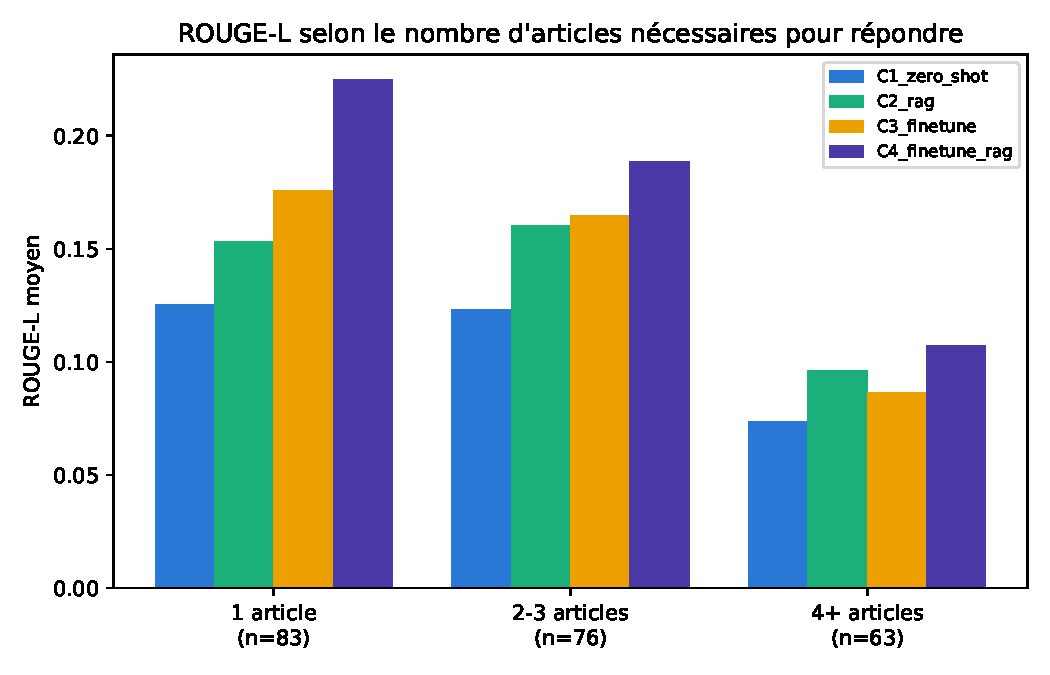
\includegraphics[width=\linewidth]{latex_assets/figs/difficulty_bucket_rouge.pdf}
\caption{ROUGE-L grouped by number of gold articles required.}
\label{fig:difficulty}
\end{figure}

Quality stays broadly stable for questions needing one to three articles and drops clearly once four or more are needed, in every configuration without exception, and neither retrieval nor fine-tuning corrects this on its own. A simple classifier was also trained to predict, before generation, whether a given question is likely to get a correctly cited answer, using only information available in advance such as question length and category. It separates reliable from unreliable questions considerably better than chance, and the same features driving that prediction, mainly question length and how common the category is in the training data, point toward the same conclusion, that some questions are foreseeably harder before the model ever generates anything.

\section{A Domain Specialist Adapter}

Looking at results broken down by legal category suggested a natural question, whether an adapter trained only on one domain would do better on that domain than the general purpose adapter. A specialist adapter was trained on the subset of training questions concerning the Code Civil, using fewer examples than the generalist adapter since that subset is smaller, and compared against the generalist on the same test questions.

The result came out mixed rather than as a clear win for specialization. On its own domain the specialist is marginally better on lexical overlap but hallucinates noticeably more, and combined with retrieval it does worse than the generalist in both domains while hallucinating less in both. Because the specialist was trained on fewer examples than the generalist, this comparison mixes together the effect of narrowing the domain with the effect of simply having less training data, and the fine-tuning results earlier in this report already show that fewer examples alone lower quality. This experiment does not really settle whether domain specialization helps, it mainly shows that a fair test of the idea needs matched training set sizes, which is planned as a follow up.

\section{Comparing Against Human Judgment}

Every measurement so far is automatic, and an automatic score can be consistent with itself while still not matching what a person would actually prefer to read. The two authors, together with a third annotator whose data collection is still ongoing, blindly compared the retrieval configuration against the fine-tuned configuration over 60 questions, without knowing which side was which.

\begin{table}[H]
\centering
\small
\begin{tabular}{lcc}
\toprule
\textbf{Annotator} & \textbf{Prefers RAG} & \textbf{Prefers fine-tune} \\
\midrule
Annotator 1 & 70.0\% & 10.0\% \\
Annotator 2 & 55.0\% & 8.3\% \\
\bottomrule
\end{tabular}
\caption{Blind pairwise preference, 60 shared questions.}
\label{tab:arena}
\end{table}

Agreement between the two annotators on the shared questions was moderate rather than strong, which is reported honestly rather than assumed away, and is discussed a little further below. Even so, both annotators clearly and independently preferred the retrieval configuration over the fine-tuned one by a wide margin. This sits in real tension with the earlier automatic comparison on 50 questions, which had found the fine-tuned model ahead on lexical overlap. Rather than trying to explain that tension away, it is taken here as the clearest sign this month that a small sample lexical comparison and a blind human preference judgment on the same two systems do not always point the same way, which is why both are now measured side by side.

\section{Reading Through the Answers}

Beyond the numbers, reading the annotated answers directly surfaced a few patterns worth describing in their own words. The most common mistake is a reversal of legal roles, an obligation placed on the wrong party, often on question pairs that differ by a single word, married against legally cohabiting for instance, where the correct article differs in a subtle way that is easy for both retrieval and generation to miss. Invented statutory text also appears fairly often, and given that hallucination does not fully disappear even under the oracle context condition, at least part of this seems to be a general tendency of the base model rather than purely a consequence of poor retrieval. A smaller number of answers simply drift away from the question asked, usually when a retrieved passage is topically close but does not actually answer what was asked. A last pattern, repeated or cut off text in some answers, looks like a decoding setting issue rather than a modelling limitation, since generation currently uses no repetition penalty, and fixing this is a small, concrete task for next month rather than an open research question.

One limitation raised by the annotators themselves deserves to be said plainly, neither is a trained legal professional, and telling a subtly wrong legal claim apart from a correct one can be genuinely hard to verify from the shortened context shown during annotation. This is a real limit of the human evaluation as it stands, not something to hide, and it is part of why the moderate agreement between annotators above should not be read as carelessness.

\section{Practical Difficulties This Month}

As in the previous report, the more time consuming technical problems are listed here briefly rather than as a narrative. The statutory article identifiers in the dataset turned out not to be uniformly numeric, a meaningful share follow regional formats and a smaller share carry a leftover artefact from how the data was originally collected, both of which had to be cleaned before any citation based metric could be trusted. No validation split existed for fine-tuning before this month, which made it impossible to tell a model that generalizes from one that memorizes on a few hundred examples, and a small fixed validation set was added specifically to close that gap. Because each computation this month runs as an independent script rather than sharing code, a fix applied in one place, most usefully saving intermediate results after every step of a long job rather than only at the end, did not carry over automatically to the others and had to be reapplied by hand. Finally, the free GPU quota used for these experiments allows only two jobs running at once, and a job that is pushed again after a bug fix does not automatically stop the earlier, still running version of itself, which caused more than one avoidable delay before this was understood.

\section{What Is Left Before the Final Report}

Three things carry over directly into next steps. The retrieval discrepancy described early in this report needs to be resolved or at least narrowed down. The third annotator's data collection and a more formal double annotated reading of the errors, only sketched qualitatively here, need to be finished. Generation should also be rerun with a repetition penalty added, to check how much of the repeated or cut off text problem described above is simply a fixable setting rather than a real limitation of the current models and data.

\begin{thebibliography}{9}

\bibitem{hu2022lora}
E. J. Hu et al.
\textit{LoRA: Low-Rank Adaptation of Large Language Models.}
ICLR 2022. arXiv:2106.09685.

\bibitem{dettmers2023qlora}
T. Dettmers et al.
\textit{QLoRA: Efficient Finetuning of Quantized LLMs.}
NeurIPS 2023. arXiv:2305.14314.

\bibitem{lewis2020rag}
P. Lewis et al.
\textit{Retrieval-Augmented Generation for Knowledge-Intensive NLP Tasks.}
NeurIPS 2020. arXiv:2005.11401.

\bibitem{bouvard2024derby}
C. Bouvard, M. Ciancone, A. Gourru, M. Schaeffer.
\textit{Derby LLM: Evaluation comparative des approches RAG et fine-tuning.}
APIA 2024. hal-04638460.

\bibitem{louis2021bsard}
A. Louis, G. Spanakis.
\textit{A Statutory Article Retrieval Dataset in French.}
ACL 2021. arXiv:2108.11792.

\bibitem{zhang2020bertscore}
T. Zhang, V. Kishore, F. Wu, K. Q. Weinberger, Y. Artzi.
\textit{BERTScore: Evaluating Text Generation with BERT.}
ICLR 2020. arXiv:1904.09675.

\bibitem{ovadia2023finetune}
O. Ovadia, M. Brief, M. Mishaeli, O. Elisha.
\textit{Fine-Tuning or Retrieval? Comparing Knowledge Injection in LLMs.}
arXiv:2312.05934, 2023.

\end{thebibliography}

\end{document}
